\documentclass[14pt]{extarticle}
\input{external/preamble-latex-cools.tex}
\begin{document}
\begin{project}{Actividad de cierre}{Expresiones para un rectángulo.}{cool-expresionesParaRectangulo}%
\begin{sidebyside}{2}{0}{0}{0}%
\begin{sbspanel}{0.6}%
%
\begin{enumerate}[label={(\alph*)}]
\item{}Marca o colorea este rectángulo para mostrar una estrategia que ayude a encontrar su área.%
\item{}Escribe una o más expresiones que representen cómo encuentras el área.%
\end{enumerate}
\end{sbspanel}%
\begin{sbspanel}{0.4}%
\includegraphics[max width=\linewidth, center]{external/svg-source/tikz-file-158678-scale13.pdf}
\end{sbspanel}%
\end{sidebyside}%
\begin{image}{0}{1}{0}{}%
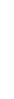
\includegraphics[max width=\linewidth, center]{external/whitespace-tikz/2cm.pdf}
\end{image}%
\end{project}
\end{document}